\chapter{Sistemas Não Lineares}
\label{chapter:cap3}
\section{\textbf{Introdução}}

\section{\textbf{Modelo de \textit{Lorenz}}}
\begin{figure}[H]
%     \centering
    \begin{subfigure}{.5\textwidth}
    \centering
    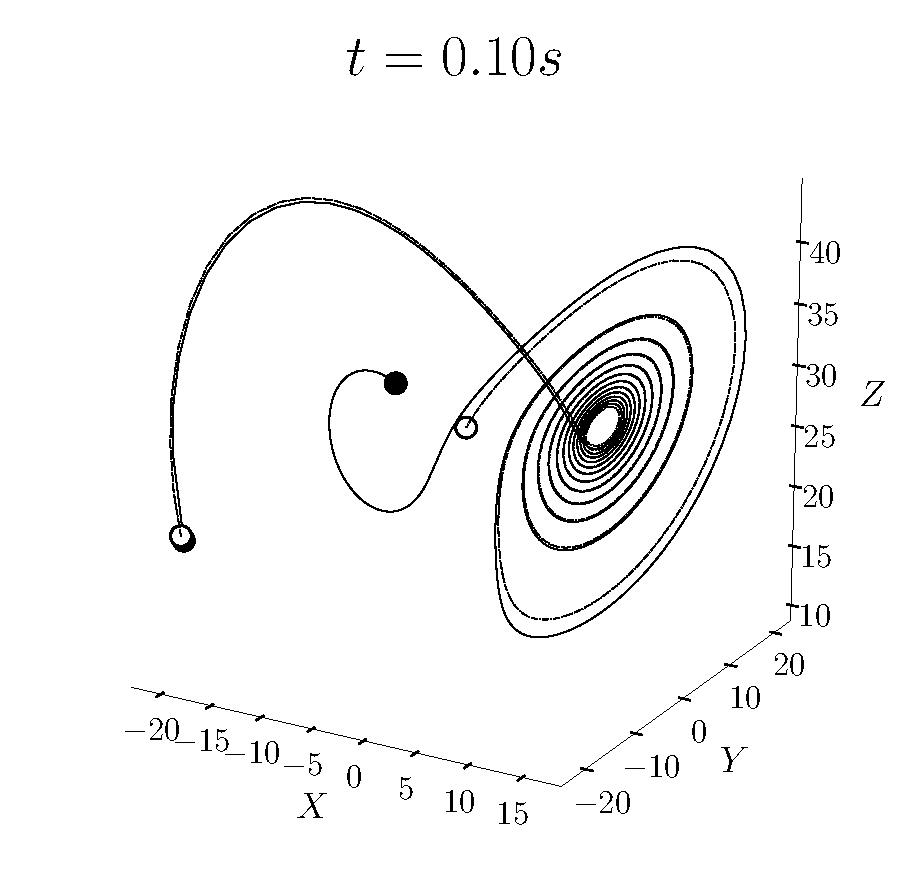
\includegraphics[width=1.\linewidth, angle=0, clip]{03_Cap3/figures/Lorenzatractor0_10.pdf}
    \end{subfigure}
    \begin{subfigure}{.5\textwidth}
    \centering
    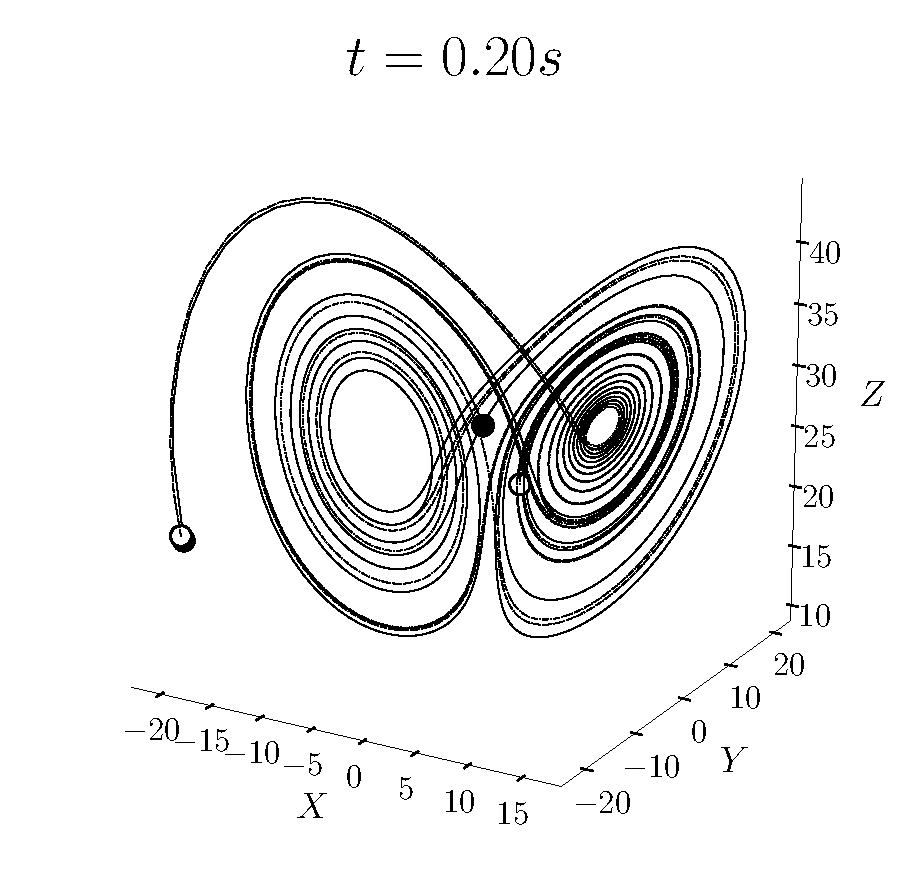
\includegraphics[width=1.\linewidth, angle=0, clip]{03_Cap3/figures/Lorenzatractor0_20.pdf}
    \end{subfigure}
    \vspace{-0.5cm}
\end{figure}
\section{\textbf{Mecanismo de reações: \textit{Brusselator}}}
O Mecanismo proposto por Prigogine e Levefer em 1968 consiste na sequência de reações em \ref{brureactions}, da qual, através da \textit{Lei de Ação das Massas}, obtemos o sistema de equações diferenciais ordinárias \ref{brusys}:\\
\begin{minipage}{.48\textwidth}
\vspace{-3ex}
\begin{align}
\hspace{-10pt}
\centering
\overline{A}&\ce{->T[\ce{$k_1$}]}\overline{X} \nonumber\\
\overline{B}+\overline{X}&\ce{->T[\ce{$k_2$}]}\overline{Y}+\overline{D} \nonumber\\
2\overline{X}+\overline{Y}&\ce{->T[\ce{$k_3$}]}3\overline{X} \nonumber\\
\overline{X}&\ce{->T[\ce{$k_4$}]}\overline{E} 
\label{brureactions}
\end{align}
\end{minipage}
\begin{minipage}{.04\textwidth}
\vspace{-3ex}
\end{minipage}
\begin{minipage}{.48\textwidth}
\vspace{-3ex}
\begin{equation}
\centering
%\text{simult\'aneas:}\quad
    \begin{dcases}
      \frac{d\overline{X}}{dt}=k_{1}\overline{A}-(k_{2}\overline{B}+k_{4})\cdot\overline{X}+k_{3}\overline{X}^2\cdot\overline{Y}\\
      \frac{d\overline{Y}}{dt}=k_{2}\overline{B}\cdot\overline{X}-k_{3}\overline{X}^2\cdot\overline{Y}\\
    \end{dcases}
%     \quad
%     \Leftrightarrow
%     \quad
%     x=1,~y=1
\label{brusys}
\end{equation}
\end{minipage}
\\[2ex]
% $\!$\\
% \vspace{2ex}
Admensionalizando as equações da forma a seguir, obtemos:
\begin{equation*}
\centering
    \begin{dcases}
      \frac{dX}{dt}=A-(B+1)X+X^2Y\\
      \frac{dY}{dt}=BX-X^2Y\\
    \end{dcases}
\end{equation*}

\subsection{Análise de estabilidade linear}
\textcolor{red!}{Escrever análise, condição de estabilidade, ponto fixo e regimes estáveis, instáveis, focos estáveis, instáveis.... }

\begin{figure}[H]
%     \centering
    \begin{subfigure}{.5\textwidth}
    \centering
    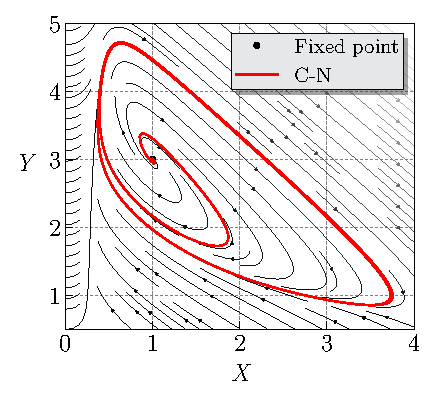
\includegraphics[width=1.\linewidth, angle=0, clip]{03_Cap3/figures/Phase_Space_internal__Brusselator__CN.pdf}
    \end{subfigure}
    \begin{subfigure}{.5\textwidth}
    \centering
    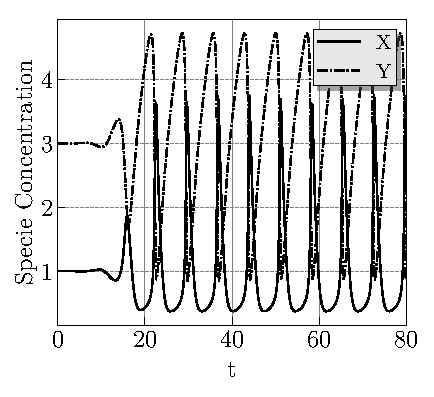
\includegraphics[width=1.\linewidth, angle=0, clip]{03_Cap3/figures/Temporal_evolution_internal__Brusselator__CN.pdf}
    \end{subfigure}
    \vspace{-0.5cm}
\end{figure}
\begin{figure}[H]
% 	\centering
	\vspace{-0.5cm}
    \begin{subfigure}{.5\textwidth}
    \centering
    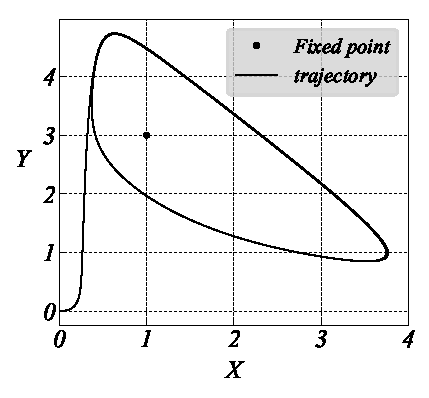
\includegraphics[width=1\linewidth, angle=0, clip]{03_Cap3/figures/Phase_Space_external__Brusselator__CN.pdf}
    \end{subfigure}
    \begin{subfigure}{.5\textwidth}
    \centering
    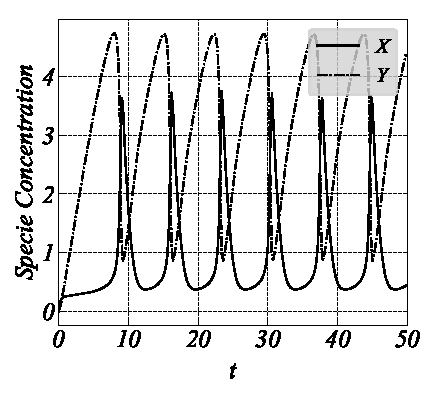
\includegraphics[width=1\linewidth, angle=0, clip]{03_Cap3/figures/Temporal_evolution_external__Brusselator__CN.pdf}
    \end{subfigure}
    \vspace{-0.5cm}
\end{figure}



\section{\textbf{Equação de \textit{Van der Pol}}}
\textcolor{red!}{(Ver Appendix 3 do Murray, Jordan and Smith 1987, Liénard Equation)}\par
A equação de \textit{Van der Pol} modela matematicamente um oscilador cujo termo de amortecimento é não linear. A equação diferencial ordinária de $2^{a}$ ordem (\ref{vanderpol}) pode ser subdividida em um sistema de EDO's de $1^{a}$ ordem (\ref{vanderpolsys}).
\begin{equation}
\ddot{x}+\epsilon (x^{2}-1)\dot{x}+x=0
\label{vanderpol}
\end{equation}
\begin{equation}
\centering
    \begin{dcases}
      \frac{dx}{dt}=y\\
      \frac{dy}{dt}=\epsilon (1-x^{2})y-x\\
    \end{dcases}
\label{vanderpolsys}
\end{equation}



\begin{figure}[H]
% 	\centering
	\vspace{-0.5cm}
    \begin{subfigure}{.5\textwidth}
    \centering
    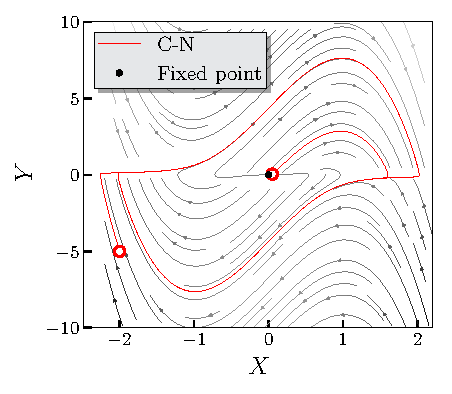
\includegraphics[width=1.\linewidth, angle=0, clip]{03_Cap3/figures/VanderPol2__Phase_Space_ep5.pdf}
    \end{subfigure}
    \begin{subfigure}{.5\textwidth}
    \centering
    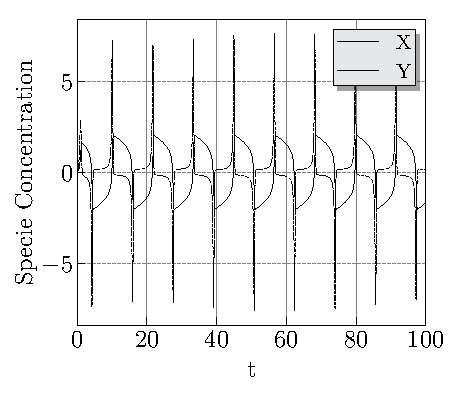
\includegraphics[width=1.\linewidth, angle=0, clip]{03_Cap3/figures/VanderPol2__2nd_Time_Evolution_ep5.pdf}
    \end{subfigure}
    \vspace{-0.5cm}
\end{figure}


% Equação...
% \begin{figure}[H]
%     \begin{subfigure}{.5\textwidth}
%     \centering
%     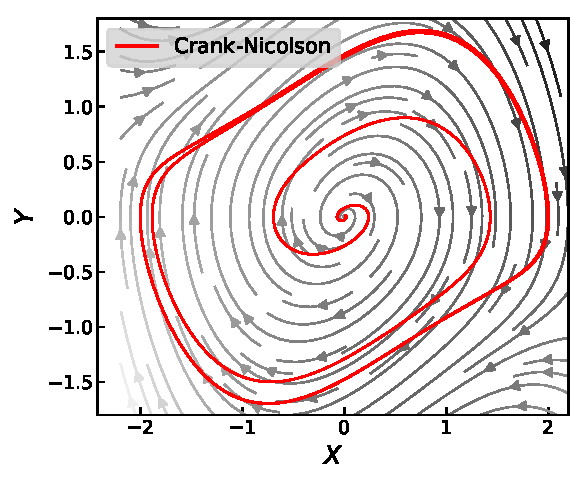
\includegraphics[width=1.0\linewidth, angle=0, clip]{02_Cap2/figures/VanderPol__Phase_Space_.pdf}
%     \end{subfigure}
%     \begin{subfigure}{.5\textwidth}
%     \centering
%     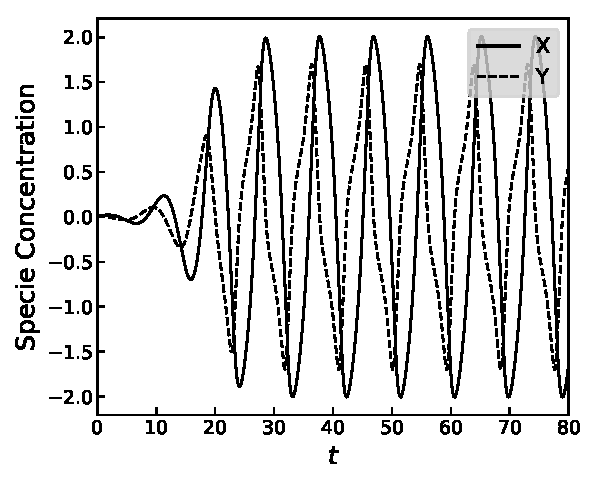
\includegraphics[width=1.0\linewidth, angle=0, clip]{02_Cap2/figures/VanderPol__Time_Evolution_.pdf}
%     \end{subfigure}
%     \vspace{-0.5cm}
% \end{figure}
% \begin{figure}[H]
%     \begin{subfigure}{.5\textwidth}
%     \centering
%     \includegraphics[width=1.0\linewidth, angle=0, clip]{02_Cap2/figures/VanderPol2__Phase_Space_.pdf}
%     \end{subfigure}
%     \begin{subfigure}{.5\textwidth}
%     \centering
%     \includegraphics[width=1.0\linewidth, angle=0, clip]{02_Cap2/figures/VanderPol2__Time_Evolution_.pdf}
%     \end{subfigure}
%     \vspace{-0.5cm}
% \end{figure} 

\section{\textbf{Modelo de \textit{Fitz-Hugh Nagumo}}}
Um dos modelos estudados extensivamente em neurobiologia e utilizado para teoria de membranas nervosas de Hodgkin-Huxley.





